% Exam Template for San Jacinto Community College Math Department courses
%Copyright@Chandi Bhandari
%%%%%%%%%%%%%%%%%%%%%%%%%%%%%%%%%%%%%%%%%%%%%%%%%%%%%%%%%%%%%%%%%%%%%%%%%%%%%%%%%%%%%%%%%%%%%%

% These lines can probably stay unchanged, although you can remove the last
% two packages if you're not making pictures with tikz.
\documentclass[11pt]{exam}
\RequirePackage{amssymb, amsfonts, amsmath, latexsym, verbatim, xspace, setspace}
\RequirePackage{tikz, pgflibraryplotmarks}
\usepackage{graphicx}
\graphicspath{ {./images/} }

% By default LaTeX uses large margins.  This doesn't work well on exams; problems
% end up in the "middle" of the page, reducing the amount of space for students
% to work on them.
\usepackage[margin=1in]{geometry}


% Here's where you edit the Class, Exam, Date, etc.
\newcommand{\class}{Math 2412 Pre-Calculus}
\newcommand{\term}{Summer 2018}
\newcommand{\examnum}{Exam III}
\newcommand{\examdate}{July, 2018}
\newcommand{\timelimit}{90 Minutes}

% For an exam, single spacing is most appropriate
\singlespacing
% \onehalfspacing
% \doublespacing

% For an exam, we generally want to turn off paragraph indentation
\parindent 0ex

\begin{document} 

% These commands set up the running header on the top of the exam pages
\pagestyle{head}
\firstpageheader{}{}{}
\runningheader{\class}{\examnum\ - Page \thepage\ of \numpages}{\examdate}
\runningheadrule

\begin{flushright}
\begin{tabular}{p{3.2in} r l}
\textbf{\class} & \textbf{\term} & \textbf{\examnum}\\
\textbf{G-Number-} & \textbf{Name (Print):}  \makebox[1.2in]{\hrulefill}\\
%\textbf{Time: \timelimit} % & \makebox[2in]{\hrulefill}

\end{tabular}\\
\end{flushright}
\rule[1ex]{\textwidth}{.1pt}

%\bf{ Choose Any 10 questions}

\hfill


%%%%%%%%%%%%%%%%%%%%%%%%%%%%%%%%%%%%%%%%%%%%%%%%%%%%%%%%%%%%%%%%%%%%%%%%%%%%%%%%%%%%%
%For the further information 
%%%%%%%%%%%%%%%%%%%%%%%%%%%%%%%%%%%%%%%%%%%%%%%%%%%%%%%%%%%%%%%%%%%%%%%%%%%%%%%%%%%%%

\begin{questions}
\addpoints
\question[4] Simplify 
		\begin{align*}
		\frac{(3-2x)^4 (x+5)4x+(3-2x)^3 3(x+5)^2}{(3-2x)^7}
		\end{align*}

\vspace{7cm}
\question[4] Write down all the possible rational solution of $P(x)=2x^3+2x^2-24$, Use Descrates Rules to determine how many positive and negative solution does it have?

\vspace{8cm}
\question[3] Check that whether x+2 is the factor of the polynomial $P(x)=x^3+2x^2-7$, why or why not give a reason. Use the remainder theorem to compute the remainder. 
\vspace{6cm}		
\addpoints
\question[4] Consider the function $f(x)=3x-2$ then find
	\begin{align*}
	\frac{f(x+h)-f(x)}{h}
	\end{align*}.
	

\vspace{8cm}
\addpoints
\question[3] Find the quotient and remainder by using the Synthetic division for 
	\begin{align*}
	\frac{x^5+3x^3-6}{x-1}
	\end{align*}

\vspace{5cm}
\question[4] Find the domain of  $f^{-1}(x)$ for the function
\begin{align*}
f(x)=-2x+4
\end{align*}.
\vspace{8cm}


\addpoints
\question[3] Solve the equation
\begin{align*}
e^{2x}-3e^x+2=0
\end{align*}
\vspace{7cm}
\question[3] Solve the equation
\begin{align*}
log(x) + log(x-1)=log(4x)
\end{align*}
\vspace{7cm}
\question [4] Find the reference angle and 3 coterminal angles (with at least one negative) for $210^\circ$ .

\vspace{8cm}
% Question with parts
%\newpage
\addpoints
\question[3]Find the area of colored sector for the given figure. 
\begin{center}
	\includegraphics{sectorarea.png}
\end{center}
\addpoints
\question[5] Find the value of the following
\begin{parts}
\part[2] $cos(\frac{\pi}{6})$
\vspace{1cm}
\part[2]  $cot(-\frac{\pi}{3})$
\vspace{1cm}
\part[2] $sin(\frac{5\pi}{4})$
\vspace{1cm}.
\part[2]  $cot(120^\circ)$
\vspace{1cm}
\part[2] $tan(-60^\circ)$
\vspace{1cm}
\end{parts}

\newpage
\vspace{8cm}
\addpoints
\question[6] A certain species of bird was introduced in a certain county 25 years ago. Biologist observer that the population doubles every 10 years, and now the population is 13,000.   
\begin{parts}
\part What was the initial size of the bird population?
\part Estimate the bird population 5 years from now. 
\end{parts}

\vspace{9cm}
\addpoints
\question[5] Draw the graph by making the table of  $f(x)=cos^{-1}(x)$. Also, State its domain and range.



\newpage
\addpoints
\question[5] Graph the one period of $y=3tan(x-\frac{\pi}{4})$







\vspace{8cm}
\addpoints
\question[4] From the top of the 200-ft lighthouse, the angle of depression to a ship in the ocean is $30^\circ$. How far is the ship from the base of lighthouse?


\newpage
\addpoints
\question[4] Find the measure of all angles $\angle A, \angle B$ and, $\angle C$ for the following graph.
\begin{center}
	\includegraphics{cosruletr.png}
\end{center}


\vspace{8cm}
\addpoints
\question[6]  Find the domain, vertical Asymptotes, Horizontal and Oblique (slant) Asymptotes (if exit), x-intercept, y-intercept of   
\begin{align*}
f(x)=\frac{\sqrt{x-2}}{x-4}
\end{align*}
 
\vspace{8cm}
\noaddpoints
\question[4] Write down $tan(\theta)$ in terms of $cos(\theta)$ in the II quadrant. 
	\vspace{8cm}
\question[4] Find the all angle and sides. 
\begin{center}
	\includegraphics{pythagoreantr.png}
\end{center}

\vspace{10cm}
\question[4] Given 
\begin{align*}
f(x)=3x-2\quad \mbox{and} \quad g(x)=\frac{3}{2x-3}
\end{align*} 
then find i) $(f\circ g)(x)$, and its domain 

\vspace{8cm}
\noaddpoints
\question[4] Is the following sequences Arithmetic, Geometric or Neither? Find Arithmetic find the common difference $d$ and if it is Geometric find the common ration$r$.
\begin{parts}
	\part [1] 7,3,-1,-5,-9,...
	\vspace{3cm}
	\part [1] 2,3,5,8,19,27,...
	\vspace{3cm}
	\part [1] 2,8,32,128,...
	\vspace{3cm}
	\part [1] 8,-4,2,-1,$\frac{1}{2}$,...
	
\end{parts}
\vspace{8cm}
\noaddpoints
\question[4] Determine whether following infinite geometric series is convergent or divergent. if it converges, find its sum \[1+\frac{1}{3}+\frac{1}{9}+\frac{1}{27}+...\]

\vspace{8cm}
\noaddpoints
\question[4] Determine the $n^{th}$ term and partial sum of 20  terms of the series \[1+\frac{1}{3}+\frac{1}{9}+\frac{1}{27}+...\]

\vspace{8cm}
\noaddpoints
\question[4] Determine the $n^{th}$ term and 20th  terms of the sequence \[11,17,23,29,...\]
\vspace{8cm}
\noaddpoints
\question[2] Find the binomial expansion of $(2x+1)^4$.

\vspace{8cm}
\addpoints
\question[5 bonus]  Graph the following function
\begin{align*}
f(x)=3^{x-3}-2
\end{align*}
\begin{center}
	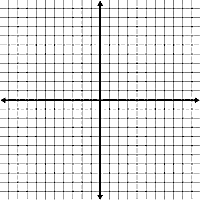
\includegraphics{graph1.png}	
\end{center}
\end{questions}
\end{document}